\documentclass[tikz,border=3.14mm]{standalone}
\usepackage{amsmath}
\begin{document}
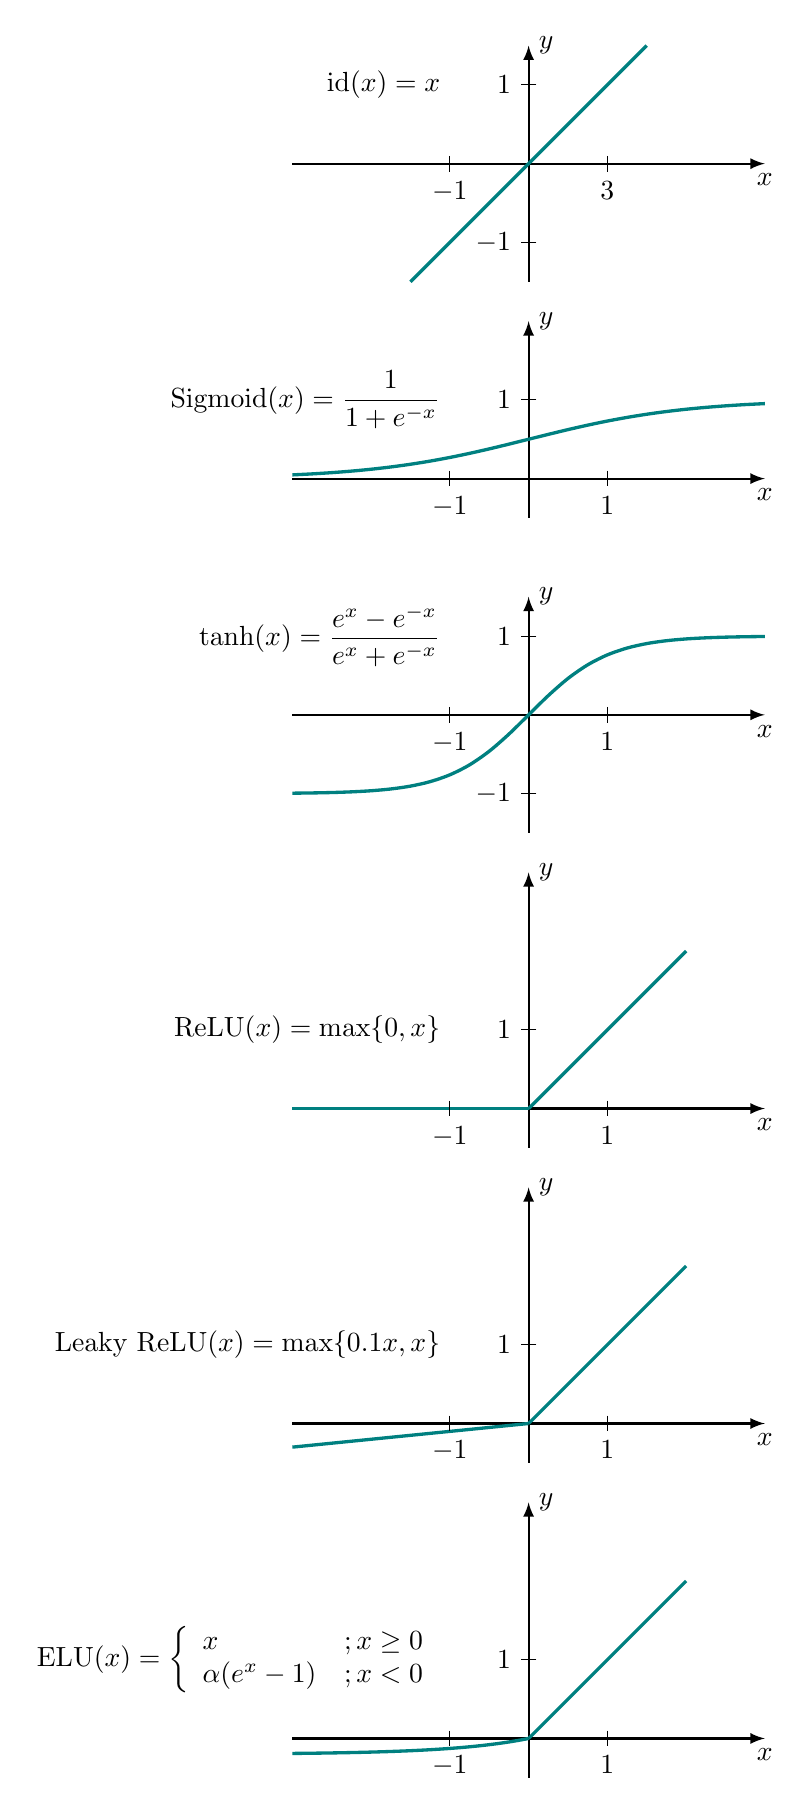
\begin{tikzpicture}[declare function={sigma(\x)=1/(1+exp(-\x));}]
    \node[left] at (-1, 1) {Sigmoid$(x) = \dfrac{1}{1+e^{-x}}$};
    \draw[thick, -latex](-3, 0) -- (3, 0) node[below] {$x$};
    \draw[thick, -latex](0, -0.5) -- (0, 2) node[right] {$y$};
    \draw[very thick, teal, domain=-3:3,smooth,variable=\t] plot ({\t}, {1/(1+exp(-\t))});
    \draw[] (-1,0.1) -- (-1, -0.1) node [below, scale=1] {$-1$};
    \draw[] (1,0.1) -- (1, -0.1) node [below, scale=1] {$1$};
    \draw[] (0.1, 1) -- (-0.1, 1) node [left] {$1$};
    \begin{scope}[yshift =+ 4cm] 
        \node[left] at (-1, 1) {$\text{id}(x) = x$};
        \draw[thick, -latex](-3, 0) -- (3, 0) node[below] {$x$};
        \draw[thick, -latex](0, -1.5) -- (0, 1.5) node[right] {$y$};
        \draw[very thick, teal, domain=-1.5:1.5,smooth,variable=\t] plot ({\t}, {\t});
        \draw[] (-1,0.1) -- (-1, -0.1) node [below, scale=1] {$-1$};
        \draw[] (1,0.1) -- (1, -0.1) node [below, scale=1] {$3$};
        \draw[] (0.1, 1) -- (-0.1, 1) node [left] {$1$};
        \draw[] (0.1, -1) -- (-0.1, -1) node [left] {$-1$};
    \end{scope}
    \begin{scope}[yshift = -3cm] 
        \node[left] at (-1, 1) {$\tanh(x) = \dfrac{e^x-e^{-x}}{e^x+e^{-x}}$};
        \draw[thick, -latex](-3, 0) -- (3, 0) node[below] {$x$};
        \draw[thick, -latex](0, -1.5) -- (0, 1.5) node[right] {$y$};
        \draw[very thick, teal, domain=-3:3,smooth,variable=\t] plot ({\t}, {tanh(\t)});
        \draw[] (-1,0.1) -- (-1, -0.1) node [below, scale=1] {$-1$};
        \draw[] (1,0.1) -- (1, -0.1) node [below, scale=1] {$1$};
        \draw[] (0.1, 1) -- (-0.1, 1) node [left] {$1$};
        \draw[] (0.1, -1) -- (-0.1, -1) node [left] {$-1$};
    \end{scope}
    \begin{scope}[yshift = -8cm] 
        \node[left] at (-1, 1) {$\text{ReLU}(x) = \max\{0, x\}$};
        \draw[thick, -latex](-3, 0) -- (3, 0) node[below] {$x$};
        \draw[thick, -latex](0, -0.5) -- (0, 3) node[right] {$y$};
        \draw[very thick, teal] (-3, 0) -- (0, 0);
        \draw[very thick, teal, domain=0:2,smooth,variable=\t] plot ({\t}, {\t});
        \draw[] (-1,0.1) -- (-1, -0.1) node [below, scale=1] {$-1$};
        \draw[] (1,0.1) -- (1, -0.1) node [below, scale=1] {$1$};
        \draw[] (0.1, 1) -- (-0.1, 1) node [left] {$1$};
    \end{scope}
    \begin{scope}[yshift = -12cm] 
        \node[left] at (-1, 1) {$\text{Leaky ReLU}(x) = \max\{0.1x, x\}$};
        \draw[thick, -latex](-3, 0) -- (3, 0) node[below] {$x$};
        \draw[thick, -latex](0, -0.5) -- (0, 3) node[right] {$y$};
        \draw[very thick, teal, domain=-3:0,smooth,variable=\t] plot ({\t}, {0.1*\t});
        \draw[very thick, teal, domain=0:2,smooth,variable=\t] plot ({\t}, {\t});
        \draw[] (-1,0.1) -- (-1, -0.1) node [below, scale=1] {$-1$};
        \draw[] (1,0.1) -- (1, -0.1) node [below, scale=1] {$1$};
        \draw[] (0.1, 1) -- (-0.1, 1) node [left] {$1$};
    \end{scope}
    \begin{scope}[yshift = -16cm] 
        \node[left] at (-1, 1) {$\text{ELU}(x) = \left\{\begin{array}{ll} x &; x\ge 0\\ \alpha (e^x-1)&; x<0\end{array}\right.$};
        \draw[thick, -latex](-3, 0) -- (3, 0) node[below] {$x$};
        \draw[thick, -latex](0, -0.5) -- (0, 3) node[right] {$y$};
        \draw[very thick, teal, domain=-3:0,smooth,variable=\t] plot ({\t}, {0.2*(exp(\t)-1)});
        \draw[very thick, teal, domain=0:2,smooth,variable=\t] plot ({\t}, {\t});
        \draw[] (-1,0.1) -- (-1, -0.1) node [below, scale=1] {$-1$};
        \draw[] (1,0.1) -- (1, -0.1) node [below, scale=1] {$1$};
        \draw[] (0.1, 1) -- (-0.1, 1) node [left] {$1$};
    \end{scope}
\end{tikzpicture}
\end{document}
